%generare il pdf con il comando: pdflatex main.tex
\documentclass[a4paper, oneside, openany,dvipsnames,table]{article}
\usepackage{../template/sos}
\usepackage{eurosym}
\usepackage{amssymb}% http://ctan.org/pkg/amssymb
\usepackage{pifont}% http://ctan.org/pkg/pifont
\usepackage{listings}
\definecolor{bluSOS}{RGB}{48, 84, 150}
\newcommand{\shellcmd}[1]{\\\indent\indent\texttt{\footnotesize\$ #1}\\}
%\WithSuffix\def\shellcmd*#1{\indent\indent\texttt{\footnotesize\$ #1}\\}
\newcommand{\Titolo}{Norme di Progetto}

\newcommand{\Gruppo}{SonsOfSwe}

\newcommand{\Redazione}{Caldart Federico, Cavallin Giovanni, Dalla Riva Giovanni, Favero Andrea, Menegon Lorenzo, Panozzo Stefano, Thiella Eleonora}

\newcommand{\ACapoRedazione}{Caldart Federico \newline Cavallin Giovanni \newline Dalla Riva Giovanni \newline Favero Andrea \newline Menegon Lorenzo \newline Panozzo Stefano \newline Thiella Eleonora}

\newcommand{\Verifica}{Caldart Federico}

\newcommand{\Approvazione}{Cavallin Giovanni}

\newcommand{\Distribuzione}{Vardanega Tullio}

\newcommand{\Uso}{interno}

\newcommand{\Data}{3 Marzo 2018}

\newcommand{\NomeProgetto}{Progetto Speect}

\newcommand{\Mail}{sonsofswe.swe@gmail.com}

\newcommand{\DescrizioneDoc}{Questo documento descrive le regole, gli strumenti e le convenzioni adottate dal gruppo SonsOfSwe durante la realizzazione del progetto Marvin.}



\begin{document}
%\copertina{}


	\begin{titlepage}
		\begin{center}

			\begin{center}
				%sostituire con immagine copertina del gruppo
				\centerline{
\includegraphics[scale=0.20]{../template/img/logo.png}}
			\end{center}

			\vspace{1cm}

			\begin{Huge}
				\textbf{\Titolo{}} \\
			\end{Huge}

			\vspace{9pt}

			\begin{large}
				\textbf{\Gruppo{}}\ - \textbf{\NomeProgetto{}}\\%\Data{}
				\vspace{6pt}
				\Mail{}
			\end{large}

			\vspace{15pt}

			\bgroup
			\def\arraystretch{1.3}
			\centering
			\begin{tabular}{r|L{5cm}}
				\multicolumn{2}{c}{\textbf{Informazioni sul documento} } \\ \hline

				\textbf{Uso} & \Uso \\
				\textbf{Distribuzione} & \Distribuzione{}
			\end{tabular}
			\egroup

			\vspace*{\fill}

			\begin{center}
				\textbf{Descrizione\\}
				\DescrizioneDoc{}
			\end{center}

		\end{center}
	\end{titlepage}

%%%%%%%%%%%%%%%%%%%%%%%%%%%%%%%%%%%%%%%%%%%%%%%%%%%%%%%%%%%%%%%%%%%%%%%%%%%%%%%%%%%%%%%%%%%%%%%%%%%%%%%
%SOMMARIO
%\definecolor{bluSOS}{RGB}{48, 84, 150}
\definecolor{greySOS}{RGB}{209, 222, 223}
\section*{Registro delle modifiche}
{
	\rowcolors{2}{greySOS}{white}
	\renewcommand{\arraystretch}{1}
	\centering
	\begin{longtable}{| c| c | C{4cm} | c | c |}
		\hline
		\rowcolor{bluSOS}
		\textcolor{white}{\textbf{Versione}} & \textcolor{white}{\textbf{Data}} & \textcolor{white}{\textbf{Descrizione}} & \textcolor{white}{\textbf{Autore}} & \textcolor{white}{\textbf{Ruolo}}\\
		\hline
		1.0.0 & 2018-04--- & Approvazione & Stefano Panozzo  & Reponsabile \\
		\hline
		0.1.0 & 2018-03-10 & Verificazione & Giovanni Cavallin  & Verificatore \\
		\hline
		0.0.1 & 2018-03-07 & Stesura della sezione \emph{Informazioni generali} e \emph{Riassunto della riunione} & Eleonora Thiella & Analista \\
		
	\end{longtable}

}

%\emph{Analisi dei Rischi}, \emph{Preventivo} ed \emph{Attualizzazione dei rischi}. Create le appendici \emph{A Attuazione dei rischi} e \emph{B organigramma}

%\newpage
\newpage
\tableofcontents
\newpage
\listoffigures
\newpage
\listoftables
\newpage
%%%%%%%%%%%%%%%%%%%%%%%%%%%%%%%%%%%%%%%%%%%%%%%%%%%%%%%%%%%%%%%%%%%%%%%%%%%%%%%%%%%%%%%%%%%%%%%%%%%%%%%
%PARAGRAFI
\hypersetup{linkcolor=bluSOS}
\newpage
\section{Introduzione}
\subsection{Scopo del documento}
Questo documento contiene la pianificazione delle attività che saranno svolte dai membri del gruppo \Gruppo{} per realizzare il progetto \NomeProgetto. In particolare, questo documento contiene:

\begin{itemize}
	\item Analisi e trattamento dei rischi;
	\item Il preventivo delle risorse necessarie allo svolgimento del progetto;
	\item Il consuntivo delle attività finora svolte.
\end{itemize}

\subsection{Scopo del prodotto}
Lo scopo del prodotto è quello di realizzare un prototipo di Uniweb come ÐApp che giri su rete Ethereum. I tre attori principali che si rapportano con Marvin sono:
\begin{itemize}
	\item Università;
	\item Professori;
	\item Studenti.
\end{itemize} 
Il portale deve quindi permettere agli studenti di accedere alle informazioni riguardanti le loro carriere universitarie, di iscriversi agli esami, di accettare o rifiutare voti e di poter vedere il loro libretto universitario.
Ai professori deve invece essere permesso registrare i voti degli studenti.
L'università ogni anno crea una serie di corsi di laurea rivolti a studenti, dove ognuno di essi comprende un elenco di esami disponibili per anno accademico. Ogni esame ha un argomento, un numero di crediti e un professore associato. Gli studenti si iscrivono ad un corso di laurea e tramite il libretto elettronico mantengono traccia ufficiale del progresso.

\subsection{Glossario}
Nel documento \textit{Glossario} i termini tecnici, gli acronimi e le abbreviazioni sono definiti in modo chiaro e conciso, in modo tale da evitare ambiguità e massimizzare la comprensione dei documenti.
\newline I vocaboli presenti in esso saranno posti in corsivo e presenteranno una "G" maiuscola a pedice.

\subsection{Riferimenti}
\subsubsection{Normativi}
\begin{itemize}
	\item \textbf{Norme di Progetto: }\textit{Norme di Progetto v1.0.0};
	\item \textbf{Capitolato d'appalto C6: \NomeProgetto}:\\
	\url{http://www.math.unipd.it/~tullio/IS-1/2017/Progetto/C6.pdf};
	\item \textbf{Regolamento del progetto didattico}:\\
	\url{http://www.math.unipd.it/~tullio/IS-1/2017/Dispense/P01.pdf};
	\item \textbf{Vincoli di organigramma e dettagli tecnico-economici}:\\
	\url{http://www.math.unipd.it/~tullio/IS-1/2017/Progetto/RO.html}.
\end{itemize}
\subsubsection{Informativi}
\begin{itemize}
	\item \textbf{Studio di Fattibilità: }\textit{Studio di Fattibilità v1.0.0};
	\item \textbf{Analisi dei Requisiti: }\textit{Analisi dei Requisiti v1.0.0};
	\item \textbf{Software Engineering (10th edition) - Ian Sommerville}:
	\begin{itemize}
		\item Chapter 2: Software processes;
		\item Chapter 22: Project management;
		\item Chapter 23: Project Planning.
	\end{itemize}
	\item \textbf{Slides del corso di Ingegneria del Software}:\\
	\url{http://www.math.unipd.it/~tullio/IS-1/2017/}.
\end{itemize}

\subsection{Modello di sviluppo}
Il modello di sviluppo scelto per il progetto è quello incrementale.\\
Durante i primi periodi, grazie ad un'analisi del capitolato e la comunicazione con il proponente, si fissano i requisiti che il sistema dovrà soddisfare e quali invece sono considerati opzionali, benchè desiderabili. Questo permette di individuare quali dei requisiti hanno una maggior importanza strategica; pertanto questi verranno soddisfatti per primi, mentre gli altri saranno adempiti successivamente.\\
Il modello infatti prevede rilasci multipli successivi, dunque è possibile sottoporre al proponente un prototipo con le funzionalità di primaria importanza nel minor tempo possibile, così da permettere una valutazione in corso d’opera del lavoro svolto. Partendo da questo prototipo sarà poi possibile effettuare un incremento delle funzionalità e un consolidamento di quelle già presenti.\\
Per ottenere ciò nel modo più efficiente ed efficace possibile, si prevede la scomposizione dello sviluppo in attività, al termine delle quali è prevista una milestone (interna o esterna). In questo modo le risorse vengono concentrate in un numero limitato di sottoattività parallele, ottenendo come risultato una loro migliore gestione e verifica.
Questo permette un maggiore controllo sulle tempistiche e sui costi in quanto ogni sottoinsieme deve essere precedentemente pianificato; ciò riduce inoltre il rischio di ritardi.\\
Infine, per ogni attività si prevedono dei giorni di slack prima della consegna dei documenti per accedere alle revisioni di avanzamento, in modo da mitigare eventuali ritardi causati da fattori non prevedibili.

\subsection{Scadenze}\label{Scadenze}
Il gruppo \Gruppo ha deciso di rispettare le seguenti scadenze:
\begin{itemize}
	\item \textbf{Revisione dei Requisiti (RR)}: 23-04-2018;
	\item \textbf{Revisione di Progettazione (RP)}: 14-05-2018;
	\item \textbf{Revisione di Qualifica (RQ)}: 15-06-2018;
	\item \textbf{Revisione di Accettazione (RA)}: 16-07-2018.
\end{itemize}

\newpage
%%%%%%%%%%%%%%%%%%%%%%%%%%%%%%%%%%%%%%%%%%%%%%%%%%%%%%%%%%%%%%%%%%%%%%%%%%%%%%%%%%%%%%%%%%%%%%%%%%%%%%%
\section{Requisiti di sistema}
Per l'installazione e l'utilizzo di questo software sono richiesti alcuni prerequisiti:
\begin{itemize}
	\item Browser web Google Chrome (aggiornato alla versione 60 o superiori) o Mozilla Firefox (aggiornato alla versione 50 o superiori);
	\item Plugin Metamask (aggiornato alla versione 4.7.1 o superiori) per i browser di cui sopra; \\
	\url{https://metamask.io/}
	\item Git \\
	\url{https://git-scm.com/downloads}
	\item Python aggiornato alla versione 2.7; \\
	\url{https://www.python.org/downloads/}
	\item Node package manager alla versione 6, e Node alla 8.11.2 \\
	\url{https://nodejs.org/it/}
	\item Nel caso si utilizzi Windows sarà necessario installare \textit{windows-build-tools} digitando nella powershell: 
	\begin{lstlisting}
		npm install --global --production windows-build-tools
	\end{lstlisting}

	 
\end{itemize}
\newpage
\section{Installazione ed esecuzione}
Il codice relativo alla Product Baseline lo si può trovare al seguente link:
\begin{center}
	\url{linkAllaRepo}
\end{center}
Una volta fatto il clone della repository o dopo aver scaricato lo zip, sono necessari i seguenti passi per far partire l'applicazione:
\begin{enumerate}
	\item Posizionarsi nella root della repo ed eseguire nella shell:
		\begin{lstlisting}
	npm install -g ganache-cli
	npm install -g truffle
	npm i
		\end{lstlisting}
	\item In seguito sempre nella shell:
		\begin{lstlisting}
	./startBlockchain.ps1
		\end{lstlisting}
	\item Infine è necessario eseguire:
		\begin{lstlisting}
	./loadProject.ps1
		\end{lstlisting}
\end{enumerate}

A questo punto noterai che il tuo browser predefinito ha aperto automaticamente l'homepage.
Ora dovrai connetteri a Metamask: nel tuo browser clicca sull'icona di Metamask e accetta l'informativa sulla privacy e le condizioni d'uso. Poi clicca su \textbf{Main Network} e scegli \textbf{Custom RPC}, inserisci nel primo form \textbf{http://localhost:9545} come in Figura~\ref{fig:metamask1} e clicca su  \textbf{Save}.
%Now you have to connect MetaMask: in your browser click on the MetaMask icon and accept the Privacy Notice and the Terms of use. Then click on \textbf{Main Network} and choose \textbf{Custom RPC}, type in the first form \textbf{http://localhost:9545} as in Figure~\ref{fig:metamask1} and click \textbf{Save}.

\begin{figure}[h]
\centering
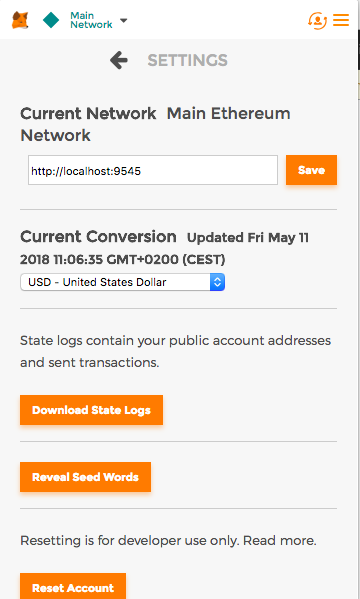
\includegraphics[height=3in]{./img/settings.png}
\caption{Setta l'RPC inserendo \textbf{http://localhost:9545}}
\label{fig:metamask1}
\end{figure}

Ora, come in Figura~\ref{fig:metamask2}, clicca su \textbf{Import Existing DEN} e (vedi Figura~\ref{fig:metamask3}) inserisci la frase \textbf{candy maple cake sugar pudding cream honey rich smooth crumble sweet treat} e la password che vuoi usare per il tuo account.


\begin{figure}[h]
\centering
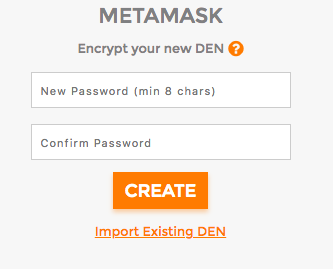
\includegraphics[height=1.8in]{./img/importa.png}
\caption{Clicca su \textbf{Import Existing DEN}}
\label{fig:metamask2}
\end{figure}

\begin{figure}[h]
\centering
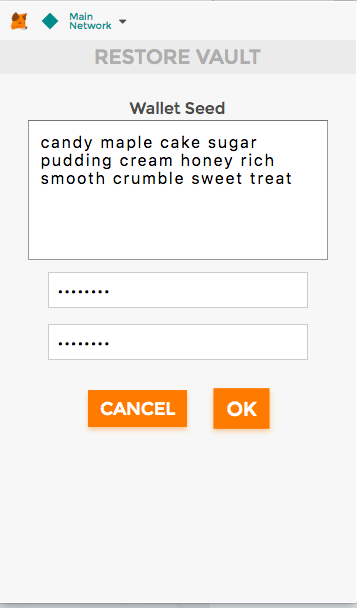
\includegraphics[height=3in]{./img/stringa_psw.png}
\caption{Inserisci la seed phrase e la password che vuoi usare}
\label{fig:metamask3}
\end{figure}



\clearpage
\newpage
\section{Confronto con la Poc}
In precedenza è stato realizzata una \emph{Proof of Concept} in cui si è data dimostrazione delle tecnologie che si sarebbero dovute utilizzare per la realizzazione del progetto Marvin.
Tale produzione è disponibile all'indirizzo: \url{https://github.com/SOS-SonsOfSwe/Marvin-PoC}.
Durante la ricerca di strumenti adatti allo scopo il team ha deciso inizialmente di basare la prima produzione del prodotto sul framework \emph{Truffle}, dal momento che esso presentava molte delle tecnologie di interesse.
Con uno studio più approfondito del pacchetto il gruppo si è reso conto che esso era una buona base di partenza per la realizzazione di un prodotto più complesso, sebbene necessitasse di alcune correzioni strutturali. Qui di seguito si elencano i limiti riscontrati e le soluzioni adottate:
\newline
\newline

\begin{table}[hp]
	\centering
\begin{tabular}{|p{6cm}|p{6cm}|}
	\hline
	\textbf{Proof of Concept} & \textbf{Product Baseline} \\
	
	\hline Architettura ben strutturata ma male incapsulata
	&
	Organizzazione migliore della struttura del pacchetto
	a fronte di una conoscenza più approfondita del design pattern MVVM e di altri su cui il framework si basa \\ 
	
	\hline Interfaccia povera e strutturata in maniera confusionaria, non chiara e  difficilmente intuibile 
	&
	Ristrutturazione completa e incremento dell'interfaccia utente, ora provvista di tutte le parti atte alla soddisfazione della maggior parte dei requisiti opzionali e obbligatori \\ 
	
	\hline Database solidity estremamente scarno e con poche funzionalità di sicurezza e di ottimizzazione
	&
	Strutturazione avanzata del backend di solidity, desisamente più ottimizzato e performante; implementazione già in fase di completamento\\
	
	\hline
\end{tabular}
\caption{Confronto tra Proof of Concept e Product Baseline}
\end{table}
\newpage
\section{Architettura del prodotto}
Dopo un approfondito studio il team ha optato per l'utilizzo del design pattern \textbf{Model View View-Model}, che prevede tre macrosezioni:
\begin{itemize}
	\item \textbf{Model}: rappresenta i dati contenuti nel sito, ma non i comportamenti o i servizi che manipolano l'informazione. Non è responsabile della renderizzazione;
	\item \textbf{View}: si occupa di rappresentare le informazioni contenute nel sito ed è quello con cui l'utente interagisce; la view in questo design pattern è attiva, al contrario di quello che succede nell'MVC, questo perché contiene comportamenti, eventi e riferimenti a stati del sito, che quindi presuppongo una conoscenza della logica che sta dietro ai dati;
	\item \textbf{Viewmodel}: fornisce i dati dal Model in una forma in cui la View può usufruirne. Si occupa inoltre della logica della vista e di mantenersi costantemente sincronizzato con la View.
\end{itemize}
Per poter apprezzare questa suddivisione nel pacchetto del team viene riportato qui di seguito il diagramma generale dei package. Si proseguirà successivamente alla descrizione delle implementazioni di ogni sezione in relazione all'architettura della Product Baseline, illustrandone i rispettivi design pattern utilizzati.
\\Per facilitare la comprensione della struttura dei diagrammi delle classi, il team ha deciso di raggruppare tutti i \emph{Containers}, i \emph{Components} e le \emph{actions} nei loro rispettivi packages. Infatti il comportamento di ogni classe di ogni package è modulare:
\begin{itemize}
	\item Tutti i \emph{Components} importano la classe \emph{React.Component}
	\item Tutti i \emph{Containers} importano il rispettivo \emph{Component}, la rispettiva \emph{Action} e il pacchetto \emph{react-redux}.
	\item Tutte le \emph{actions} importano le \emph{costants} che azionano il \emph{reducer}, il pacchetto \emph{react-router}, lo \emph{store}, il pacchetto \emph{truffle-contract} e la classe \emph{IpfsUtils}
\end{itemize}
I diagrammi presentati in questo documento illustrano la struttura sinteticamente; la loro versione integrale si può trovare nella cartella XXX.

%diagramma dei package generale




\subsection{View}
\subsubsection{Design patterns}
Progettando questa sezione ci si è resi conto che si sarebbero potute generare delle classi \emph{dumb}, ovvero slegate dalla logica del sistema e che si sarebbero dovute occupare solamente della rappresentazione delle informazioni. Per ottenere questo si è ricorso all'utilizzo del seguente design pattern:
\begin{itemize}
	\item \textbf{Decorator}: sfruttando il macro-package \emph{Container}, che poi si occupa di collegare il componente allo stato di \emph{redux}, si possono decorare tutte le componenti ivi presenti con dei componenti react puri, ai quali vengono passate eventualmente le informazioni e le funzioni a disposizione attraverso un accesso al \emph{this.props}. In questa maniera si ha la completa separazione tra rappresentazione e dati - cosa auspicata dal framework MVVM - e si facilitano modifiche future.
\end{itemize}

\subsubsection{Diagramma delle classi}
In seguito è riportato il diagramma delle classi relativo a questa sezione con evidenziato la posizione del design pattern utilizzato:

%diagramma con vista su View

\subsection{ViewModel}
\subsubsection{Design patterns}
Progettando questa sezione ci si è resi conto che si sarebbero potute generare delle classi \emph{dumb}, ovvero slegate dalla logica del sistema e che si sarebbero dovute occupare solamente della rappresentazione delle informazioni. Per ottenere questo si è ricorso all'utilizzo del seguente design pattern:
\begin{itemize}
	\item \textbf{Observer}: descrizione per quanto riguarda il comportamento di trigger-client che opera Redux sullo stato di React
	\item \textbf{Facade}: per generare un'interfaccia astratta dalle implementazioni delle classi che poi si vanno ad utilizzare.
	\item \textbf{Adapter}: per interagire col model si usa un adaptator offerto dal framework truffle che si occupa di fare-un-sacco-di-cose-belle-da-chiedere-a-Stefano
	\item \textbf{Command}: come redux ordina a react di re-renderizzare le pagine al cambiamento dello state dovuto ad un dispatch di un'azione
\end{itemize}

\subsubsection{Diagramma delle classi}
In seguito è riportato il diagramma delle classi relativo a questa sezione con evidenziato la posizione del design pattern utilizzato:

%diagramma con vista su View


\newpage
\section{Requisiti soddisfatti}
\subsection{Tabella del soddisfacimento dei requisiti}
\begin{table}[hp]
\centering
\begin{tabular}{|c|c|c|}
\hline
ID requisito & Soddisfacimento nell'architettura & Soddisfacimento nel codice \\ \hline
R0F1         & SODDISFATTO                       & SODDISFATTO                \\ \hline
R0F2         & SODDISFATTO                       & SODDISFATTO                \\ \hline
R0F3         & SODDISFATTO                       & SODDISFATTO                \\ \hline
R0F4        & SODDISFATTO                       & SODDISFATTO                \\ \hline
R0F5        & SODDISFATTO                       & SODDISFATTO                \\ \hline
R0F6        & SODDISFATTO                       & SODDISFATTO                \\ \hline
R2F7        & SODDISFATTO                       & NON SODDISFATTO                \\ \hline
R2F8        & SODDISFATTO                       & NON SODDISFATTO                \\ \hline
R2F9        & SODDISFATTO                       & NON SODDISFATTO                \\ \hline
R2F10        & SODDISFATTO                       & NON SODDISFATTO                \\ \hline
R2F11        & SODDISFATTO                       & NON SODDISFATTO                \\ \hline
R2F13        & SODDISFATTO                       & NON SODDISFATTO                \\ \hline
R2F14        & SODDISFATTO                       & NON SODDISFATTO                \\ \hline
R0F15        & SODDISFATTO                       & SODDISFATTO                \\ \hline
R0F16        & SODDISFATTO                       & SODDISFATTO                \\ \hline
R0F17        & SODDISFATTO                       & SODDISFATTO                \\ \hline
R0F18        & SODDISFATTO                       & SODDISFATTO                \\ \hline
R0F19        & SODDISFATTO                       & NON SODDISFATTO                \\ \hline
R2F20        & SODDISFATTO                       & NON SODDISFATTO                \\ \hline
R2F21        & SODDISFATTO                       & NON SODDISFATTO                \\ \hline
R2F22        & SODDISFATTO                       & NON SODDISFATTO                \\ \hline
R0F23        & SODDISFATTO                       & SODDISFATTO                \\ \hline
R0F24        & SODDISFATTO                       & SODDISFATTO                \\ \hline
R2F25        & SODDISFATTO                       & NON SODDISFATTO                \\ \hline
R0F26        & SODDISFATTO                       & SODDISFATTO                \\ 
\hline
\end{tabular}
\caption{Requisiti soddisfatti}
\end{table}
\clearpage

\subsection{Grafici sui requisiti soddisfatti}
\begin{figure}[hp]
\centering
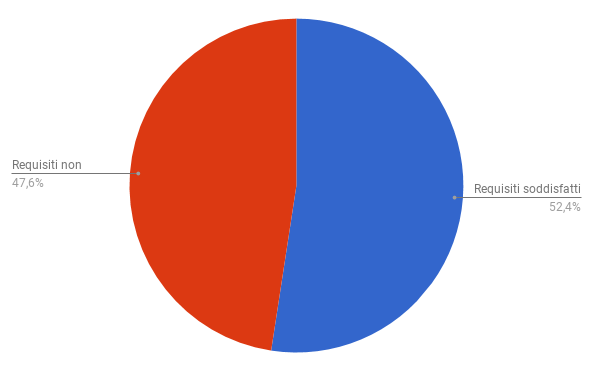
\includegraphics[height=7cm]{img/RequisitiSoddisfatti.png}\\
\caption{Requisiti soddisfatti}
\end{figure}

\begin{figure}[hp]
\centering
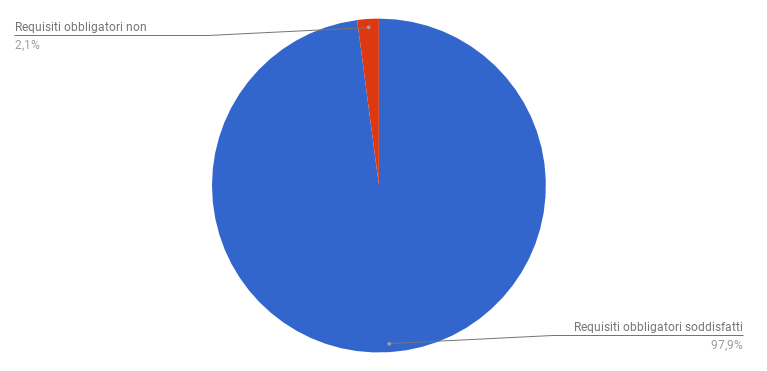
\includegraphics[height=7cm]{img/RequisitiObbligatoriSoddisfatti.png}\\
\caption{Requisiti obbligatori soddisfatti}
\end{figure}

\pagebreak
\section{Casi d'uso soddisfatti}
\subsection{Tabella del soddisfacimento dei casi d'uso}
\begin{table}[hp]
\centering
\begin{tabular}{|c|c|c|}
\hline
ID caso d'uso & Soddisfacimento nell'architettura & Soddisfacimento nel codice \\ \hline
UC1         & SODDISFATTO                       & NON SODDISFATTO                \\ \hline
UC2         & SODDISFATTO                       & NON SODDISFATTO                \\ \hline
UC3         & SODDISFATTO                       & NON SODDISFATTO                \\ \hline
UC4         & SODDISFATTO                       & NON SODDISFATTO                \\ \hline
UC6         & SODDISFATTO                       & SODDISFATTO                \\ \hline
UC7         & SODDISFATTO                       & SODDISFATTO                \\ \hline
UC8         & SODDISFATTO                       & SODDISFATTO                \\ \hline
UC9         & SODDISFATTO                       & SODDISFATTO                \\ \hline
UC10         & SODDISFATTO                       & SODDISFATTO                \\ \hline
UC11         & SODDISFATTO                       & NON SODDISFATTO                \\ \hline
UC12         & SODDISFATTO                       & NON SODDISFATTO                \\ \hline
UC13         & SODDISFATTO                       & NON SODDISFATTO                \\ \hline
UC14         & SODDISFATTO                       & NON SODDISFATTO                \\ \hline
UC15         & SODDISFATTO                       & NON SODDISFATTO                \\ \hline
UC16         & SODDISFATTO                       & NON SODDISFATTO                \\ \hline
UC17         & SODDISFATTO                       & NON SODDISFATTO                \\ \hline
UC18         & SODDISFATTO                       & NON SODDISFATTO                \\ \hline
UC19         & SODDISFATTO                       & NON SODDISFATTO                \\ \hline
UC20         & SODDISFATTO                       & NON SODDISFATTO                \\ \hline
UC21         & SODDISFATTO                       & NON SODDISFATTO                \\ \hline
UC22         & SODDISFATTO                       & NON SODDISFATTO                \\ \hline
UC23         & SODDISFATTO                       & SODDISFATTO                \\ \hline
UC24         & SODDISFATTO                       & NON SODDISFATTO                \\ \hline
UC25         & SODDISFATTO                       & NON SODDISFATTO                \\ \hline
UC26         & SODDISFATTO                       & NON SODDISFATTO                \\ \hline
UC27         & SODDISFATTO                       & SODDISFATTO                \\ \hline
UC28         & SODDISFATTO                       & SODDISFATTO                \\ \hline
UC29         & SODDISFATTO                       & NON SODDISFATTO                \\ \hline
UC30         & SODDISFATTO                       & SODDISFATTO                \\ \hline
UC31         & SODDISFATTO                       & SODDISFATTO                \\ \hline
UC32         & SODDISFATTO                       & SODDISFATTO                \\ \hline
UC33         & SODDISFATTO                       & SODDISFATTO                \\ \hline

\end{tabular}
\caption{Casi d'uso soddisfatti}
\end{table}
\clearpage

\subsection{Grafici sui casi d'uso soddisfatti}
\begin{figure}[hp]
\centering
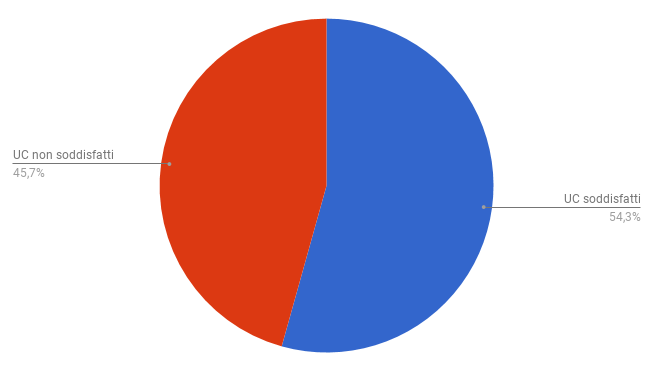
\includegraphics[height=7cm]{img/UCSoddisfatti.png}\\
\caption{Casi d'uso soddisfatti}
\end{figure}



\end{document}


